\chapter{Организация параллельных вычислений в модели общей циркуляции океана}\label{ch:inmsom/ch2}

\section{Реализация параллельной версии модели}\label{sec:inmsom/ch2/sec1}
    В качестве основной идеи распараллеливания сигма-модели INMOM используется метод декомпозиции области.
    Разбиение на подобласти происходит только в горизонтальной плоскости, игнорируя вертикальную плоскость (см. рис. \ref{fig:ddm3d}). 
    Причин этому несколько: во-первых, слой океана имеет небольшую толщину по сравнению с горизонтальными масштабами и поэтому вертикальное измерение можно игнорировать
	при разбиении на подобласти.
	И во-вторых, по вертикали в сигма-модели используется всегда одно и то же количество
	расчетных уровней, а значит можно рассматривать метод балансировки нагрузки вычислений с использованием фрактальных кривых только в горизонтальной плоскости.
%	и оптимальность полученного разбиения будет точно соответствовать оптимальности для трехмерной сигма-модели INMOM.

    %Процессор проводит вычисления только на своей подобласти  и если ему понадобятся данные с соседней подобласти, то осуществляется обмен данными между процессорами.    
    После разбиения на подобласти для каждой подобласти добавляется внерасчётная граница толщиной в одну узловую точку. 
    В начале каждого расчета происходит синхронизация между процессорами для обновления значений на внерасчётных границах.
    При синхронизации пограничные блоки процессора помещаются во внерасчётные границы своих соседних процессоров.
    Когда процессор в своих вычислениях подходит к границе своей подобласти и ему требуются данные с соседней подобласти - он берет эти данные 
    со своей внерасчётной границы и продолжает вычисления \cite{GuansuoWang}.
   
    
    В качестве базового алгоритма разбиения расчётной области используется равномерное разбиение на прямоугольные подобласти \cite{ChaplyginINMOM2017}.     
    Рассмотрим расчётную область, состоящую из множества точек $\{ (i, j, k) : 1 \leq i \leq n_x,  1 \leq j \leq n_y, 1 \leq k \leq n_z \}$,
    где $n_x$, $n_y$, $n_z$ - количество точек по $x$, $y$, $z$ соответственно. 
    Пусть используется $p$ процессоров, образующих сетку $p = p_{x} \times p_{y}$,
    где $p_x$ - количество процессоров по $x$ и $p_y$ - количество процессоров по $y$. 
    Тогда при равномерном разбиении каждому процессору с координатами $(p_1, p_2)$ ставится в соответствие прямоугольная подобласть из множества точек
    $\{ (i, j, k) :  n_{x, start} \leq i \leq n_{x, end} , n_{y, start} \leq j \leq n_{y, end}, 1 \leq k \leq n_z \}$, где:  
    
    \begin{equation} \label{eq:inmsom/a9} 
    \begin{array}{c} 
    \displaystyle{ n_{x, start} = \lceil \frac{n_x}{p_x} \rceil (p_1 - 1) + 1 ~,~ n_{x, end} =  \lceil \frac{n_x}{p_x} \rceil (p_1) } \\	
    
    \displaystyle{ n_{y, start} = \lceil \frac{n_y}{p_y} \rceil (p_2 - 1) + 1 ~,~ n_{y, end} =  \lceil \frac{n_y}{p_y} \rceil (p_2) }
    \end{array}
    \end{equation} 
    
	\begin{figure}[htb!]
	\center
	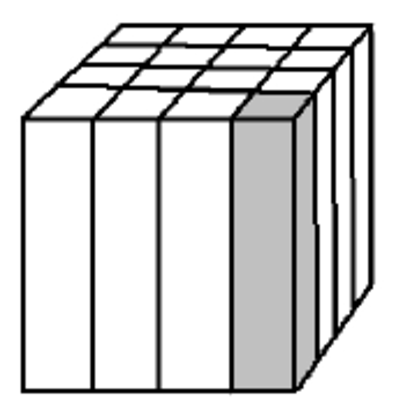
\includegraphics[scale = 0.4]{domain_decomposition.png}
	\caption{Метод декомпозиции области в горизонтальной плоскости}
	\label{fig:ddm3d}
	\end{figure}
        
    Также в сигма-модели INMOM реализована декомпозиция на более сложные области: произвольные прямоугольные многоугольники. 
    Для этого в модели был реализован блочный подход.
    Исходная область равномерно разбивается на прямоугольные блоки, границы блоков рассчитываются по формулам (\ref{eq:inmsom/a9}). 
    Далее, каждому процессору ставятся в соответствие некоторое количество блоков, которые и формируют расчётную подобласть процессора. 
    Блочный подход был подробно описан в главе \ref{sec:ch2/sec2} применительно к модели мелкой воды. Для модели общей циркуляции океана эта техника обобщается на трехмерное пространство, сохраняя все преимущества блочного подхода и для сигма-модели океана. 		
    Перечислим эти преимущества блочного подхода применимо к сигма-модели океана INMOM.
    Во-первых, это возможность проводить декомпозицию на более сложные области, обеспечивающую балансировку нагрузки на процессоры. 
    Во-вторых, выбирая оптимальные размеры блока можно получить ускорение модели за счет попадания каждого блока в кэш память.
    В-третьих, данный подход довольно несложно программно реализуем и поэтому его внедрение в такой сложный код, как сигма-модель океана INMOM, происходило 
    без существенных изменений.

    Похожий блочный подход уже зарекомендовал себя в таких моделях океана, как Parallel Ocean Program (POP) \cite{POP}, \cite{gmd-7-267-2014} и HIROMB (High Resolution Operational Model for the Baltic Sea) \cite{HIROMB}.
    
    Синхронизация внерасчётных границ блоков реализована с помощью неблокирующих вызовов MPI\_Isend, MPI\_Irecv,
    причём, если соседние блоки расположены на одном процессоре, то вызовов MPI процедур не происходит - вместо этого
    происходит обычное копирование с границы одного блока на внерасчётную границу другого блока. 
    Также возможно использование гибридного подхода MPI + OpenMP, где каждый OpenMP поток обрабатывает по блоку.
    Процедуры чтения/записи в модели INMOM реализованы средствами MPI-IO,
    которые позволяют процессорам осуществлять параллельную чтение/запись файлов,
    объединяя запросы на чтение/запись от нескольких процессоров в один,
    что существенно ускоряет процесс \cite{ChaplyginINMOM2017}, \cite{TerehovINMOM2010}.
    
    Как уже было сказано ранее в главе \ref{sec:inmsom/ch1/sec2}, в сигма-модели океана INMOM на этапе баротропной адаптации возникает линейная система алгебраических уравнений, которую необходимо решать на каждом шаге по времени. Для этого нужно использовать параллельный решатель линейных систем. 
    В параллельной сигма-модели INMOM для этих целей используется библиотека PETSc (Portable, Extensible Toolkit for
Scientific Computation) \cite{PETSc}.
    Данная библиотека обладает очень гибким функционалом и большим разнообразием
    параллельных решателей линейных систем и предобуславливателей для них.
    В качестве базового параллельного решателя линейной системы (\ref{eq:inmsom/20}) 
    используется GMRES,  в качестве предобуславливателя - аддитивный метод Шварца (ASM: Additive Schwarz Method) с предобуславливателем ILU(k) для каждого блока в матрице.
    Параметр перекрытия для предобуславливателя ASM был выбран единицей.
    Предобуславливатель ASM по своей природе отлично подходит для параллельных вычислений,
    но тем не менее обладает одним
    недостатком: число обусловленности предобусловленной системы увеличивается с уменьшением размера блоков матрицы: $\kappa \leq C(1 + d/\delta)/d^2$, где $k$ - число обусловленности, $d$ - размер блока матрицы, $\delta$ - параметр перекрытия метода. % missing cite
     Поэтому в качестве блоков матрицы выбираются подобласти процессоров целиком, а не блоки из которых состоят подобласти.
    %Это сделано, чтобы число итераций решателя не увеличивалось еще сильнее при переходе на большее количество процессоров.
    
    В таблице представлено сравнение количества итераций и времени решения системы (\ref{eq:inmsom/20})
    в зависимости от параметра k у предобуславливателя ILU(k), который используется при решении для каждого блока матрицы. Тестирование проводилось на 16 процессорах для акватории Азовского моря с разрешением 250 метров, сеточная область размером $1525 \times 1115$ точек. Проводилось 72 шага с шагом по времени 30 секунд и в таблице представлены средние значения итераций решателя и времени, затраченные на решение одного шага по времени.      
    Таблица демонстрирует насколько важен выбор правильного предобуславливателя для каждого блока матрицы. Для рассмотренной задачи ILU(4) показал наилучшие результаты поэтому в дальнейшем мы будем использовать именно его.
    
    Следует отметить, что выбранная связка линейного решателя и предобуславливателя
    для системы (\ref{eq:inmsom/20}) не обязательно является оптимальной,
    но тем не менее успела зарекомендовать себя во многих расчетах.
    Нахождение оптимальной связки уже выходит за рамки нашей работы и 
    поэтому этот вопрос опускается.

\bigskip

\begin{table}[htb!]
\caption{Количество итераций и время решения решателя GMRES в связке с ASM в зависимости от выбора предобуславливателя ILU(k) для каждого блока матрицы.}
\begin{tabular}{|c|c|c|c|c|c|}
\hline 
Preconditioner & ILU(0) & ILU(2) & ILU(4) & ILU(8) & ILU(16) \\ 
\hline 
Average iterations & 50 & 16 & 14 & 13 & 14 \\ 
\hline 
Average time (sec) & 1.29 & 0.46 & 0.45 & 0.61 & 0.84 \\ 
\hline 
\end{tabular} 
\end{table}

    %В качестве основного средства распараллеливания используется технология MPI. 
    %Так же возможно использование гибридного подхода MPI + OpenMP. В этом случае происходит декомпозиция области
    %и на каждой подобласти используется технология распараллеливания OpenMP, обмен данными между процессорами происходит с помощью технологии MPI.


	В модели общей циркуляции океана был реализован метод балансировки нагрузки вычислений с использованием кривых Гильберта, подробно описанный в \ref{sec:ch2/sec3} применительно к модели мелкой воды. Важно отметить, что оптимальность разбиения для мелкой воды точно соответствует оптимальности для трехмерной сигма-модели INMOM, так как количество расчетных уровней по глубине в ней одинаково для всех точек сетки по горизонтали. Это позволяет без особых изменений реализовать предложенный алгоритм балансировки нагрузки вычислений на процессорах для модели общей циркуляции океана INMOM.

\FloatBarrier
